\documentclass[aspectratio=169]{beamer}

% Thème et couleurs personnalisées
\usetheme{Madrid}
\usecolortheme{default}

% Palette de couleurs CECI
\definecolor{ceciblue}{RGB}{0, 102, 153}
\definecolor{cecilight}{RGB}{102, 178, 204}
\definecolor{cecidark}{RGB}{0, 51, 102}
\definecolor{accentgreen}{RGB}{0, 153, 102}
\definecolor{codebg}{RGB}{245, 245, 245}

\setbeamercolor{palette primary}{bg=ceciblue,fg=white}
\setbeamercolor{palette secondary}{bg=cecilight,fg=white}
\setbeamercolor{palette tertiary}{bg=cecidark,fg=white}
\setbeamercolor{palette quaternary}{bg=accentgreen,fg=white}
\setbeamercolor{structure}{fg=ceciblue}
\setbeamercolor{section in toc}{fg=ceciblue}

% Packages nécessaires
\usepackage[utf8]{inputenc}
\usepackage[T1]{fontenc}
\usepackage{listings}
\usepackage{tikz}
\usepackage{hyperref}
\usepackage{multirow}
\usepackage{booktabs}

% Style pour les blocs de code
\lstdefinestyle{bashstyle}{
    backgroundcolor=\color{codebg},
    basicstyle=\ttfamily\footnotesize,
    breaklines=true,
    commentstyle=\color{accentgreen},
    keywordstyle=\color{ceciblue}\bfseries,
    stringstyle=\color{cecidark},
    frame=single,
    rulecolor=\color{cecilight},
    numbers=left,
    numberstyle=\tiny\color{gray},
    xleftmargin=2em,
    framexleftmargin=1.5em
}

\lstset{style=bashstyle}

% Pied de page personnalisé
\setbeamertemplate{footline}{
  \leavevmode%
  \hbox{%
  \begin{beamercolorbox}[wd=.33\paperwidth,ht=2.25ex,dp=1ex,center]{author in head/foot}%
    \usebeamerfont{author in head/foot}\insertshortauthor
  \end{beamercolorbox}%
  \begin{beamercolorbox}[wd=.34\paperwidth,ht=2.25ex,dp=1ex,center]{title in head/foot}%
    \usebeamerfont{title in head/foot}\insertshorttitle
  \end{beamercolorbox}%
  \begin{beamercolorbox}[wd=.33\paperwidth,ht=2.25ex,dp=1ex,right]{date in head/foot}%
    \usebeamerfont{date in head/foot}\insertshortdate{}\hspace*{2em}
    \insertframenumber{} / \inserttotalframenumber\hspace*{2ex}
  \end{beamercolorbox}}%
  \vskip0pt%
}

% Informations du titre
\title[CECI HPC Introduction]{Getting Started with CECI\\High-Performance Computing}
\subtitle{A Practical Guide}
\author{Guillaume Deside}

\date{\today}

\begin{document}

% --- Page de titre ---
\begin{frame}
  \titlepage
  \begin{center}
    \small
     High-Performance Computing for Research
  \end{center}
\end{frame}

% --- Table des matières ---
\begin{frame}{Outline}
  \tableofcontents
\end{frame}

\section{Introduction to CECI}

\begin{frame}{What is CECI?}
\begin{columns}[T]
\column{0.55\textwidth}
\textbf{Consortium des Équipements de Calcul Intensif}

\vspace{0.8em}
\textcolor{ceciblue}{\textbf{A Belgian Federation for HPC}}

\vspace{0.5em}
\begin{itemize}
    \item Federation of Belgian university HPC centers
    \item Shared computational infrastructure
    \item Available to \textbf{all Belgian researchers}
    \item 5 major clusters across Belgium
    \item Combined: \textbf{12,688 cores} + \textbf{56 GPUs}
    \item Coordinated access and support
\end{itemize}

\column{0.45\textwidth}
\begin{block}{Why Use HPC?}
\begin{itemize}
    \item \textbf{Massive parallelization}\\
    {\small Thousands of cores}
    \item \textbf{Large memory capacity}\\
    {\small Up to 2 TB per node}
    \item \textbf{Long-running computations}\\
    {\small Up to 21 days}
    \item \textbf{GPU acceleration}\\
    {\small Latest RTX/A-series}
    \item \textbf{Big data storage}\\
    {\small Up to 520 TB}
    \item \textbf{Specialized software}\\
    {\small Pre-installed modules}
\end{itemize}
\end{block}
\end{columns}
\end{frame}

\begin{frame}{CECI Clusters Overview}
\begin{table}
\centering
\scriptsize
\begin{tabular}{lllrrlll}
\toprule
\textbf{Cluster} & \textbf{University} & \textbf{CPU} & \textbf{Cores} & \textbf{Memory} & \textbf{Network} & \textbf{Storage} & \textbf{Max Time} \\
\midrule
\textbf{Lyra} & ULB & Genoa 3.25 GHz & 1,280 & 128 GB & 50 GbE & CephFS 500 TB & 5 days \\
\textbf{Lemaitre4} & UCLouvain & Genoa 2.4 GHz & 5,120 & 766 GB & HDR Ib & BeeGFS 320 TB & 2 days \\

\textbf{NIC5} & ULiège & Rome 2.9 GHz & 4,672 & 256 GB-1 TB & HDR Ib & BeeGFS 520 TB & 2 days \\

\textbf{Hercules2} & UNamur & Naples 2 GHz & 1,024 & 256 GB-2 TB & 10 GbE & NFS 80 TB & 15 days \\

\textbf{Dragon2} & UMons & SkyLake 2.6 GHz & 592 & 192-384 GB & 10 GbE & RAID0 3.3 TB & 21 days \\
\bottomrule
\end{tabular}
\end{table}

\vspace{0.3em}

\centering
\url{https://www.ceci-hpc.be/clusters.html}
\begin{exampleblock}{Key Infrastructure}
\begin{itemize}
    \item AMD Genoa/Rome/Naples/SkyLake
    \item HDR InfiniBand (MPI clusters)
    \item Large-scale storage (80-520 TB)
    \item Latest GPU architectures
\end{itemize}
\end{exampleblock}


\end{frame}

% ============================================
% SECTION 2: Getting Access & Connecting
% ============================================
\section{Getting Access \& Connecting}

\begin{frame}{Step 1: Create Your CECI Account}
\begin{block}{Account Creation}
Visit: \url{https://login.ceci-hpc.be/init/}
\end{block}

\begin{columns}[T]
\column{0.5\textwidth}
\textbf{What You'll Need:}
\begin{itemize}
    \item University email address
    \item Choose a passphrase
    \item Institutional affiliation
\end{itemize}



\column{0.5\textwidth}
\textbf{What You'll Receive:}
\begin{itemize}
    \item Confirmation email
    \item Your CECI username
    \item \textbf{Private SSH key}: \texttt{id\_rsa.ceci}
\end{itemize}

\vspace{0.5em}
\begin{exampleblock}{Next Step}
Download and securely store your \texttt{id\_rsa.ceci} key file
\end{exampleblock}
\end{columns}

\vspace{0.5em}
\centering
\textcolor{ceciblue}{\textbf{Keep your private key secure and never share it!}}
\end{frame}

\begin{frame}{Step 2: Configure Your Computer}
\begin{center}
\Large \textcolor{ceciblue}{\textbf{Different procedures for different operating systems}}
\end{center}

\vspace{1em}
\begin{columns}[T]
\column{0.30\textwidth}
\begin{block}{\centering Windows}
\centering
\vspace{0.5em}
\textbf{MobaXterm}\\
{\small (Recommended)}
\vspace{0.3em}
\begin{itemize}
    \item Free SSH client
    \item File transfer
    \item Session manager
\end{itemize}
\end{block}

\column{0.30\textwidth}
\begin{block}{\centering Mac / Linux}
\centering

\vspace{0.5em}
\textbf{Terminal + SSH}\\
{\small (Built-in)}
\vspace{0.3em}
\begin{itemize}
    \item Native SSH support
    \item Configure \texttt{.ssh/config}
    \item Simple setup
    \item Command-line
\end{itemize}
\end{block}

\column{0.30\textwidth}
\begin{block}{\centering VS Code}
\centering
\vspace{0.5em}
\textbf{Remote SSH}\\
{\small (All platforms)}
\vspace{0.3em}
\begin{itemize}
    \item Visual interface
    \item Integrated terminal
    \item File explorer
    \item Code editing
\end{itemize}
\end{block}
\end{columns}

\vspace{1em}
\centering
\textcolor{ceciblue}{Choose the method that works best for your workflow!}
\end{frame}

\begin{frame}{Windows: MobaXterm Setup}
\begin{columns}[T]
\column{0.5\textwidth}
\textbf{Installation \& Configuration:}
\begin{enumerate}
    \item Download MobaXterm from\\
    {\small \url{https://mobaxterm.mobatek.net/}}
    \item Install the free Home Edition
    \item Import your \texttt{id\_rsa.ceci} key
    \item Configure SSH session with gateway
\end{enumerate}

\vspace{0.5em}
\begin{exampleblock}{Video Tutorial}
Complete setup walkthrough:\\
\url{https://www.youtube.com/watch?v=o41r0mFaURU}
\end{exampleblock}

\column{0.45\textwidth}
\begin{alertblock}{Key Settings}
\begin{itemize}
    \item \textbf{Gateway:}\\
    {\small \texttt{gwceci.cism.ucl.ac.be}}
    \item \textbf{Username:}\\
    {\small Your CECI login}
    \item \textbf{Private key:}\\
    {\small \texttt{id\_rsa.ceci}}
    \item \textbf{Cluster:}\\
    {\small \texttt{lemaitre4.cism.ucl.ac.be}}
\end{itemize}
\end{alertblock}
\end{columns}

\vspace{0.5em}
\centering
\textcolor{ceciblue}{\textbf{MobaXterm simplifies gateway + cluster access}}
\end{frame}

\begin{frame}[fragile]{Mac/Linux: SSH Setup (1/3)}
\textbf{1. Store Your Private Key}

\begin{lstlisting}[language=bash]
# Create .ssh directory if it doesn't exist
mkdir -p ~/.ssh
# Move the downloaded key to .ssh folder
mv ~/Downloads/id_rsa.ceci ~/.ssh/
# Set correct permissions (IMPORTANT!)
chmod 600 ~/.ssh/id_rsa.ceci
\end{lstlisting}

\vspace{0.2em}
\begin{alertblock}{For WSL (Windows Subsystem for Linux)}
Your key might be at:\\
\texttt{/mnt/c/Users/<yourUsername>/Downloads/id\_rsa.ceci}
\end{alertblock}

\vspace{0.2em}
\begin{alertblock}{Permission Error?}
If SSH refuses the key with \texttt{"Permissions 0644 are too open"}\\
→ Make sure you ran \texttt{chmod 600}
\end{alertblock}
\end{frame}

\begin{frame}[fragile]{Mac/Linux: SSH Setup (2/3)}
\textbf{2. Create Your Public Key}

\begin{lstlisting}[language=bash]
# Generate public key from private key
ssh-keygen -yf ~/.ssh/id_rsa.ceci > ~/.ssh/id_rsa.ceci.pub
\end{lstlisting}

You'll be asked for the passphrase you chose during account creation.

\vspace{1em}
\begin{alertblock}{Error: "invalid format" or "error in libcrypto"?}
Run this command to fix line endings:
\begin{lstlisting}[language=bash]
dos2unix ~/.ssh/id_rsa.ceci
\end{lstlisting}

If \texttt{dos2unix} is not installed:
\begin{itemize}
    \item Mac: \texttt{brew install dos2unix}
    \item Linux: \texttt{sudo apt install dos2unix}
\end{itemize}
\end{alertblock}
\end{frame}

\begin{frame}[fragile]{Mac/Linux: SSH Setup (3/3)}
\textbf{3. Configure SSH Config File}

\begin{block}{Use the SSH Config Wizard}
\url{https://www.ceci-hpc.be/sshconfig.html}
\begin{enumerate}
    \item Choose your university
    \item Provide your CECI username
    \item Copy the generated configuration
\end{enumerate}
\end{block}

\textbf{4. Edit your config file:}
\begin{lstlisting}[language=bash]
# Open/create config file
nano ~/.ssh/config

# Paste the wizard output, then save (Ctrl+X, Y, Enter)

# Set correct permissions
chmod 600 ~/.ssh/config
\end{lstlisting}
\end{frame}

\begin{frame}[fragile]{Connecting to CECI Clusters}
\textbf{After configuration, connecting is simple:}

\begin{lstlisting}[language=bash]
# Connect to any cluster using the alias
ssh <cecicluster>

# Examples:
ssh lyra          # ULB
ssh lemaitre4     # UCLouvain
ssh nic5          # ULiege
ssh hercules      # UNamur
ssh dragon2       # UMons
\end{lstlisting}

\vspace{0.1em}
\begin{alertblock}{SSH Gateway}
UCLouvain users: Use \texttt{gwceci.cism.ucl.ac.be} as SSH gateway\\
See CISM documentation for details
\end{alertblock}
\end{frame}

\begin{frame}{VS Code Remote SSH}
\begin{columns}[T]
\column{0.5\textwidth}
\textbf{Setup:}
\begin{enumerate}
    \item Install VS Code
    \item Install "Remote - SSH" extension
    \item Open Command Palette (F1)
    \item Select "Remote-SSH: Connect to Host"
    \item Choose your cluster alias\\
    {\small (e.g., \texttt{lemaitre4})}
\end{enumerate}

\vspace{0.3em}
\begin{exampleblock}{Benefits}
\begin{itemize}
    \item Edit files directly on cluster
    \item Integrated terminal
    \item File explorer
    \item Git integration
\end{itemize}
\end{exampleblock}

\column{0.4\textwidth}
\begin{block}{Requirements}
\begin{itemize}
    \item SSH config already set up
    \item \texttt{id\_rsa.ceci} key configured
    \item VS Code installed locally
\end{itemize}
\end{block}

\vspace{0.5em}
\begin{alertblock}{First Connection}
VS Code will:
\begin{itemize}
    \item Install server on cluster
    \item Take a few minutes
    \item Only happens once
\end{itemize}
\end{alertblock}

\end{columns}
\end{frame}



% ============================================
% SECTION: Basic Linux Commands
% ============================================
\section{Essential Linux Commands}

\begin{frame}[fragile]{Navigation \& File System}
\begin{block}{Moving Around}
\begin{lstlisting}[language=bash]
# Print current directory
pwd
# Change directory
cd /path/to/directory
cd ~                    # Go to home directory
cd ..                   # Go up one level
# List files and directories
ls                      # Basic listing
ls -l                   # Detailed listing (permissions, size, date)
ls -lh                  # Human-readable sizes (KB, MB, GB)
\end{lstlisting}
\end{block}

\begin{exampleblock}{Quick Tip}
Use \texttt{Tab} for auto-completion of paths and filenames!
\end{exampleblock}
\end{frame}

\begin{frame}[fragile]{Creating \& Managing Files/Directories}
\begin{columns}[T]
\column{0.5\textwidth}
\textbf{Creating:}
\begin{lstlisting}[language=bash]
# Create directory
mkdir myproject
mkdir -p path/to/dir
\end{lstlisting}

\textbf{Copying:}
\begin{lstlisting}[language=bash]
# Copy file
cp file.txt backup.txt
# Copy directory
cp -r myproject/ backup/
\end{lstlisting}

\column{0.5\textwidth}
\textbf{Moving/Renaming:}
\begin{lstlisting}[language=bash]
# Move or rename
mv oldname.txt newname.txt
mv file.txt /path/to/dir/
\end{lstlisting}

\textbf{Deleting:}
\begin{lstlisting}[language=bash]
# Remove file
rm file.txt
# Remove directory
rm -r mydir/
\end{lstlisting}

\begin{alertblock}{Warning}
\texttt{rm} is permanent! No trash/recycle bin!
\end{alertblock}
\end{columns}
\end{frame}

\begin{frame}[fragile]{File Permissions with chmod}
\textbf{Understanding Permissions:}
\begin{lstlisting}[language=bash]
ls -l myfile.txt
# Output: -rwxr-xr-- 1 user group 1234 Jan 01 12:00 myfile.txt
#         -rwxr-xr--
#          ||||||||| 
#          ||||||++-- Others: r-- (read only)
#          |||+++---- Group:  r-x (read, execute)
#          +++------- Owner:  rwx (read, write, execute)
\end{lstlisting}

\vspace{0.5em}
\begin{columns}[T]
\column{0.5\textwidth}
\textbf{Numeric Method:}
\begin{lstlisting}[language=bash]
chmod 600 id_rsa.ceci
# Owner: 6 (rw-)
# Group: 0 (---)
# Other: 0 (---)
\end{lstlisting}

\column{0.5\textwidth}
\textbf{Symbolic Method:}
\begin{lstlisting}[language=bash]
chmod +x script.sh
\end{lstlisting}
\end{columns}
\end{frame}



\begin{frame}[fragile]{Disk Usage \& Storage Management}
\begin{columns}[T]
\column{0.5\textwidth}
\textbf{Check Disk Space:}
\begin{lstlisting}[language=bash]
# Show disk usage
df -h
# Check your quota
quota -s
\end{lstlisting}

\column{0.5\textwidth}
\textbf{File Compression:}
\begin{lstlisting}[language=bash]
# Compress file
gzip largefile.txt
# Creates: largefile.txt.gz
# Decompress
gunzip largefile.txt.gz
# Create tar archive
tar -czf archive.tar.gz mydir/
# Extract tar archive
tar -xzf archive.tar.gz
\end{lstlisting}
\end{columns}

\vspace{0.5em}
\begin{alertblock}{HPC Best Practice}
Compress large data files to save quota:\\
\texttt{gzip results.csv} can reduce size by 80-90\%!
\end{alertblock}
\end{frame}



% ============================================
% SECTION: SLURM Commands for Job Management
% ============================================
\section{SLURM Job Management}

\begin{frame}[fragile]{Understanding SLURM}
\begin{columns}[T]
\column{0.5\textwidth}
\textbf{What is SLURM?}
\begin{itemize}
    \item \textbf{S}imple \textbf{L}inux \textbf{U}tility for \textbf{R}esource \textbf{M}anagement
    \item Job scheduler used on CECI clusters
    \item Manages compute resources
    \item Ensures fair access for all users
    \item Queues and prioritizes jobs
\end{itemize}



\column{0.5\textwidth}
\begin{block}{Key SLURM Commands}
\begin{description}
    \item[\texttt{sinfo}] Cluster status
    \item[\texttt{sbatch}] Submit job
    \item[\texttt{squeue}] View queue
    \item[\texttt{scancel}] Cancel job
    \item[\texttt{sacct}] Job history
    \item[\texttt{srun}] Interactive job
\end{description}
\end{block}

\vspace{0.5em}
\begin{alertblock}{Remember}
Never run computationally intensive jobs on login nodes! Always use SLURM.
\end{alertblock}
\end{columns}
\end{frame}

\begin{frame}[fragile]{sinfo - Cluster Information}
\textbf{Check cluster status and available resources:}

\begin{lstlisting}[language=bash]
# Basic cluster information
sinfo
# Detailed view
sinfo -l
# Show only available nodes
sinfo -t idle
# Node-specific information
sinfo -N
\end{lstlisting}

\vspace{0.3em}
\textbf{Example Output:}
\begin{lstlisting}[language=bash]
PARTITION AVAIL  TIMELIMIT  NODES  STATE NODELIST
Def          up   2-00:00:00     40  alloc node[001-040]
Def          up   2-00:00:00     88   idle node[041-128]
gpu          up   5-00:00:00      2  alloc gpu[01-02]
gpu          up   5-00:00:00     38   idle gpu[03-40]
\end{lstlisting}

\begin{exampleblock}{Understanding the Output}
\begin{itemize}
    \item \texttt{PARTITION}: Queue type (default, gpu, etc.)
    \item \texttt{TIMELIMIT}: Maximum job duration
    \item \texttt{STATE}: \textcolor{accentgreen}{idle} (available), \textcolor{ceciblue}{alloc} (in use), \textcolor{red}{down} (offline)
\end{itemize}
\end{exampleblock}
\end{frame}

\begin{frame}[fragile]{sbatch - Submitting Batch Jobs}
\textbf{Submit a job script to the queue:}

\begin{lstlisting}[language=bash]
# Basic submission
sbatch myjob.sbatch
\end{lstlisting}

\vspace{0.5em}
\textbf{Example Job Script (\texttt{myjob.sbatch}):}
\begin{lstlisting}[language=bash]
#!/bin/bash
#SBATCH --job-name=my_analysis
#SBATCH --output=output_%j.log
#SBATCH --error=error_%j.log
#SBATCH --time=02:00:00
#SBATCH --ntasks=1
#SBATCH --cpus-per-task=4
#SBATCH --mem="16G"

# Run your code
python3 analysis.py
\end{lstlisting}
\end{frame}

\begin{frame}[fragile]{sbatch - Common SBATCH Options}
\begin{table}
\small
\begin{tabular}{ll}
\toprule
\textbf{Option} & \textbf{Description} \\
\midrule
\texttt{--job-name=NAME} & Job name (appears in queue) \\
\texttt{--output=FILE} & Standard output file (\%j = job ID) \\
\texttt{--error=FILE} & Standard error file \\
\texttt{--time=HH:MM:SS} & Maximum runtime (e.g., 02:30:00) \\
\texttt{--ntasks=N} & Number of tasks (for MPI) \\
\texttt{--cpus-per-task=N} & CPUs per task \\
\texttt{--mem=SIZE} & Memory (e.g., 16G, 32GB) \\
\texttt{--mem-per-cpu=SIZE} & Memory per CPU \\
\texttt{--partition=NAME} & Partition/queue (gpu, Def, etc.) \\
\texttt{--gres=gpu:N} & Request N GPUs \\
\texttt{--array=1-10} & Job array (10 similar jobs) \\
\texttt{--mail-user=EMAIL} & Email for notifications \\
\texttt{--mail-type=TYPE} & When to email (BEGIN, END, FAIL, ALL) \\
\bottomrule
\end{tabular}
\end{table}
\end{frame}


\begin{frame}[fragile]{squeue - View Job Queue}
\textbf{Check status of jobs in the queue:}

\begin{lstlisting}[language=bash]
# View only YOUR jobs
squeue --me
# View all jobs
squeue
# Detailed view
squeue -l
\end{lstlisting}

\vspace{0.5em}
\textbf{Example Output:}
\begin{lstlisting}[language=bash]
JOBID    NAME         USER     ST  TIME  NODES NODELIST
123456   my_analysis  jdoe     R   1:23  1     node042
123457   data_proc    jdoe     PD  0:00  1     (Priority)
\end{lstlisting}

\begin{itemize}
    \item \texttt{R} = Running, \texttt{PD} = Pending, \texttt{CG} = Completing
    \item \texttt{TIME} = How long job has been running
\end{itemize}
\end{frame}

\begin{frame}[fragile]{squeue - Understanding Job States}
\begin{table}
\small
\begin{tabular}{lll}
\toprule
\textbf{State} & \textbf{Code} & \textbf{Meaning} \\
\midrule
Running & \textcolor{accentgreen}{R} & Job is currently running \\
Pending & \textcolor{ceciblue}{PD} & Job is waiting in queue \\
Completing & \textcolor{ceciblue}{CG} & Job is finishing up \\
Completed & \textcolor{accentgreen}{CD} & Job finished successfully \\
Failed & \textcolor{red}{F} & Job failed \\
Cancelled & \textcolor{orange}{CA} & Job was cancelled \\
Timeout & \textcolor{red}{TO} & Job exceeded time limit \\
Node Fail & \textcolor{red}{NF} & Node failed during job \\
Out of Memory & \textcolor{red}{OOM} & Job exceeded memory limit \\
\bottomrule
\end{tabular}
\end{table}


\end{frame}

\begin{frame}[fragile]{scancel - Cancel Jobs}
\textbf{Cancel running or pending jobs:}

\begin{lstlisting}[language=bash]
# Cancel specific job
scancel 123456
# Cancel all YOUR jobs
scancel -u $USER
# Cancel by job name
scancel --name=my_analysis
# Cancel jobs in specific state
scancel -u $USER --state=PENDING
# Cancel job array
scancel 123456_[1-10]
# Cancel specific array task
scancel 123456_5
\end{lstlisting}

\end{frame}

\begin{frame}[fragile]{sacct - Job Accounting \& History}
\textbf{View completed and running job information:}

\begin{lstlisting}[language=bash]
# View your recent jobs
sacct
# View specific job
sacct -j 123456
# Jobs from today
sacct --starttime=today
# All jobs with specific name
sacct --name=my_analysis
# View failed jobs only
sacct --state=FAILED
\end{lstlisting}
\end{frame}


\begin{frame}[fragile]{Quick Reference: SLURM Commands}
\begin{table}
\small
\begin{tabular}{ll}
\toprule
\textbf{Command} & \textbf{Purpose} \\
\midrule
\texttt{sinfo} & View cluster status and partitions \\
\texttt{sinfo -N} & View node-level information \\
\texttt{sbatch script.sh} & Submit batch job \\
\texttt{squeue --me} & View YOUR jobs in queue \\
\texttt{squeue -u \$USER} & View YOUR jobs (alternative) \\
\texttt{squeue} & View ALL jobs in queue \\
\texttt{squeue -j 123456} & View specific job status \\
\texttt{scancel 123456} & Cancel specific job \\
\texttt{scancel -u \$USER} & Cancel ALL your jobs \\
\texttt{sacct} & View job history \\
\texttt{sacct -j 123456} & View specific job details \\
\texttt{sacct -S today} & View today's jobs \\
\bottomrule
\end{tabular}
\end{table}

\vspace{0.5em}
\centering
\textcolor{ceciblue}{\textbf{Master these commands for efficient HPC workflow!}}
\end{frame}


% ============================================
% SECTION: First example: Running a Python Script 
% ============================================
\section{Practical Example: ML gridsearch}


\begin{frame}[fragile]{Example 1: Python with Built-in Parallelization}
\textbf{Scenario:} Your Python code uses functions that parallelize internally\\
(e.g., scikit-learn's \texttt{GridSearchCV} with \texttt{n\_jobs=-1})

\begin{block}{ONE-TIME SETUP: Create Virtual Environment}
\begin{lstlisting}[language=bash]
# Create virtual environment
python3 -m venv env
# Activate environment
source env/bin/activate
pip install numpy pandas matplotlib
pip install -U scikit-learn
\end{lstlisting}
\end{block}

\begin{alertblock}{EVERY SESSION: Activate Environment}
\begin{lstlisting}[language=bash]
source env/bin/activate
\end{lstlisting}
Before running any Python code, always activate your environment first!
\end{alertblock}

\end{frame}

\begin{frame}{Example: Machine Learning with Scikit-Learn}
\begin{block}{Scenario}
Train a Random Forest model on a large dataset
\begin{itemize}
    \item Dataset: 10,000 samples, 20 features
    \item Model: Random Forest with 1000 trees
    \item Task: Hyperparameter tuning with Grid Search
\end{itemize}
\end{block}

\end{frame}

\begin{frame}[fragile]{Step 1: Python Script}
\begin{lstlisting}[language=Python]
rf = RandomForestClassifier(random_state=42)
grid_search = GridSearchCV(
    rf, param_grid, cv=5, 
    n_jobs=-1,  # Use all available cores!
    verbose=2
)
\end{lstlisting}
\end{frame}


\begin{frame}{Two Ways to Submit Jobs}
\begin{columns}[T]
\column{0.45\textwidth}
\begin{block}{Method 1: Manual SBATCH Script}
\begin{itemize}
    \item Create \texttt{.sbatch} file with SBATCH directives
    \item Submit with \texttt{sbatch script.sbatch}
    \item Good for: simple, one-time jobs
    \item Easy to understand and modify
\end{itemize}
\end{block}

\vspace{0.2em}
\textbf{Best for:}
\begin{itemize}
    \item Learning SLURM
    \item Quick experiments
\end{itemize}

\column{0.45\textwidth}
\begin{block}{Method 2: Python-Generated Scripts}
\begin{itemize}
    \item Python function creates SBATCH script
    \item Automatically submits job
    \item Good for: parameter sweeps, many jobs
    \item Programmatic job management
\end{itemize}
\end{block}

\vspace{0.2em}
\textbf{Best for:}
\begin{itemize}
    \item Batch experiments
    \item Automated workflows
\end{itemize}
\end{columns}

\vspace{0.2em}
\centering
\textcolor{ceciblue}{\textbf{Choose the method that fits your workflow!}}
\end{frame}

\begin{frame}[fragile]{Method 1: Manual SBATCH Script}
\textbf{Create a file: \texttt{example\_cpu.sbatch}}

\begin{lstlisting}[language=bash]
#!/bin/bash
#SBATCH --job-name=Example_CPU
#SBATCH --time=00:30:00
#SBATCH --ntasks=1
#SBATCH --cpus-per-task=25
#SBATCH --mem-per-cpu=400
#SBATCH --mail-user=guillaume.deside@uclouvain.be
#SBATCH --mail-type=FAIL
#SBATCH --mail-type=END
#SBATCH --output=example_CPU.txt

python3 example_ml.py
\end{lstlisting}

\vspace{0.2em}
\textbf{Submit the job:}
\begin{lstlisting}[language=bash]
sbatch example_cpu.sbatch
# Output: Submitted batch job 123456
\end{lstlisting}
\end{frame}

\begin{frame}[fragile]{Method 2: Using the Python Submission Function}
\textbf{Example: Submit CPU Job (python3 submit.py)}

\begin{lstlisting}[language=Python]
# Define job configuration
job_info = {
    "job_name": "Example_CPU",
    "time": "00:30:00",
    "ntasks": 1,
    "cpus_per_task": 25,
    "mem_per_cpu": 400,  # MB
    "mail_user": "guillaume.deside@uclouvain.be",
    "output": "example_CPU.txt",
    "script": "python3 example_ml.py"
}
# Submit the job
job_id = submit_job(job_info, "example_cpu.sbatch")
print(f"Submitted job {job_id}")
\end{lstlisting}


\end{frame}

\begin{frame}[fragile]{Real Example: Random Forest Results}
\textbf{Job submitted with 25 CPUs:}

\begin{lstlisting}[language=bash, basicstyle=\ttfamily\scriptsize]
[INFO] CPU Detection:
  - Total CPUs available: 128
  - SLURM allocated CPUs: 25
  - Using SLURM allocation
  
[STEP 1/4] Generating synthetic dataset...
[STEP 3/4] Starting Grid Search...
Fitting 5 folds for each of 8 candidates, totalling 40 fits
[STEP 4/4] Training Results:
  - Total training time: 6.56 minutes (393.9 seconds)
  - Best cross-validation score: 0.9545
  - Best parameters:
      max_depth: 20
      min_samples_split: 5
      n_estimators: 500
[PERFORMANCE METRICS]
  - Number of CPUs used: 128
  - SLURM allocation: 25 CPUs
  - Wall-clock time: 393.9 seconds
\end{lstlisting}
\end{frame}

\begin{frame}{Understanding HPC Benefits}
\begin{alertblock}{Important Note About Performance}
Modern laptops (especially M-series Macs) may have \textbf{faster CPUs} than older HPC nodes, making direct speed comparisons misleading.
\end{alertblock}

\begin{block}{Real Benefits of HPC (Beyond Raw Speed)}
\begin{enumerate}
    \item \textbf{Free Your Computer}
    \begin{itemize}
        \item Submit job and continue working
        \item No laptop battery drain
        \item No overheating concerns
    \end{itemize}
\end{enumerate}
\end{block}
\end{frame}

\begin{frame}{Real Benefits of HPC (Beyond Raw Speed)}
\begin{block}{Real Benefits of HPC (Beyond Raw Speed) - continued}
\begin{enumerate}
    \setcounter{enumi}{1}
    \item \textbf{Scale Beyond Your Hardware}
    \begin{itemize}
        \item Access 25-128 CPUs (vs your 4-8 cores)
        \item Use up to 2TB RAM (vs your 16-32GB)
        \item Access professional GPUs
    \end{itemize}
    
    \item \textbf{Run Multiple Experiments}
    \begin{itemize}
        \item Submit 10 jobs simultaneously
        \item Parameter sweeps across many configs
        \item Overnight runs without worry
    \end{itemize}
\end{enumerate}
\end{block}
\end{frame}

\begin{frame}{Laptop vs HPC: The Real Comparison}
\begin{columns}[T]
\column{0.45\textwidth}
\begin{alertblock}{Your Laptop}
\textbf{Advantages:}
\begin{itemize}
    \item Newer, faster CPU
    \item Immediate access
    \item No queue time
    \item Easy debugging
\end{itemize}

\textbf{Limitations:}
\begin{itemize}
    \item \textcolor{red}{Computer unavailable}
    \item \textcolor{red}{Limited cores (4-12)}
    \item \textcolor{red}{Limited RAM (8-32GB)}
    \item \textcolor{red}{Battery/heat issues}
    \item \textcolor{red}{One job at a time}
\end{itemize}
\end{alertblock}

\column{0.45\textwidth}
\begin{exampleblock}{HPC Cluster}
\textbf{Advantages:}
\begin{itemize}
    \item \textcolor{accentgreen}{Computer stays free}
    \item \textcolor{accentgreen}{Many cores (25-128)}
    \item \textcolor{accentgreen}{Huge RAM (up to 2TB)}
    \item \textcolor{accentgreen}{No hardware concerns}
    \item \textcolor{accentgreen}{Multiple jobs in parallel}
    \item \textcolor{accentgreen}{Professional GPUs}
\end{itemize}

\textbf{Limitations:}
\begin{itemize}
    \item Older CPUs
    \item Queue waiting time
    \item Remote access needed
\end{itemize}
\end{exampleblock}
\end{columns}

\vspace{0.5em}
\centering
\textcolor{ceciblue}{\textbf{Use HPC for scale and convenience, not just speed!}}
\end{frame}

\begin{frame}[fragile]{Practical Workflow: Parameter Sweep}
\textbf{Use Python to submit multiple jobs with different parameters:}

\begin{lstlisting}[language=Python]
cpu_configs = [1, 4, 8, 16, 32]

for n_cpus in cpu_configs:
    job_info = {
    ... (some parameters)
        "ntasks": 1,
        "cpus_per_task": n_cpus,
        "mem_per_cpu": 400,
        "output": f"rf_cpu_{n_cpus}_%j.log",
        "script": f"python3 train_rf.py --n_jobs={n_cpus}"
    }
    job_id = submit_job(job_info, f"rf_cpu_{n_cpus}.sbatch")
    print(f"Submitted job {job_id} with {n_cpus} CPUs")
\end{lstlisting}

\begin{exampleblock}{Benefit}
Test 5 configurations simultaneously instead of sequentially!
\end{exampleblock}
\end{frame}

\begin{frame}{When to Use Each Method}
\begin{table}
\small
\begin{tabular}{lll}
\toprule
\textbf{Scenario} & \textbf{Method} & \textbf{Why} \\
\midrule
Learning SLURM & Manual script & Easy to understand \\
Single experiment & Manual script & Quick and simple \\
Quick test & Manual script & Less overhead \\
\midrule
Parameter sweep & Python function & Automate variations \\
Many similar jobs & Python function & Avoid repetition \\
Complex workflows & Python function & Programmatic control \\
Job dependencies & Python function & Manage job chains \\
Production pipeline & Python function & Reproducibility \\
\bottomrule
\end{tabular}
\end{table}

\vspace{0.5em}
\begin{exampleblock}{Tip}
Start with manual scripts to learn, then transition to Python automation for complex workflows!
\end{exampleblock}
\end{frame}

% ============================================
% Section: GPU Example
% ============================================


\section{GPU Example: Deep Learning}
\begin{frame}{Example: CNN Image Classification}
\begin{block}{Scenario}
Train a Convolutional Neural Network on CIFAR-10 dataset
\begin{itemize}
    \item Dataset: 50,000 training images (32×32 pixels, 10 classes)
    \item Model: Simple CNN with 3 convolutional layers
    \item Task: Train for 20 epochs
\end{itemize}
\end{block}

\vspace{0.5em}
\begin{columns}[T]
\column{0.45\textwidth}
\begin{alertblock}{CPU (32 cores)}
\begin{itemize}
    \item Training time: \textbf{~15 minutes}
    \item Limited by sequential ops
    \item High CPU usage
\end{itemize}
\end{alertblock}

\column{0.45\textwidth}
\begin{exampleblock}{GPU (1× RTX 6000)}
\begin{itemize}
    \item Training time: \textbf{~90 seconds}
    \item Optimized for matrix ops
\end{itemize}
\end{exampleblock}
\end{columns}

\vspace{0.5em}
\centering
\textcolor{ceciblue}{\textbf{Deep Learning = GPU's sweet spot!}}
\end{frame}


\begin{frame}[fragile]{Python Script}
\begin{lstlisting}[language=Python]
import torch
import torch.nn as nn
import torch.optim as optim
from torchvision import datasets, transforms
from torch.utils.data import DataLoader
import time
import sys

# Check if GPU is available
device = torch.device("cuda" if torch.cuda.is_available() else "cpu")
print(f"Using device: {device}")
if torch.cuda.is_available():
    print(f"GPU: {torch.cuda.get_device_name(0)}")
    print(f"GPU Memory: {torch.cuda.get_device_properties(0).total_memory / 1e9:.2f} GB")

\end{lstlisting}
\end{frame}

\begin{frame}[fragile]{GPU Jobs: Special Considerations}
\begin{alertblock}{Important: GPU-Specific Setup}
GPU jobs require CUDA-compatible packages and correct partition selection
\end{alertblock}

\vspace{0.5em}
\begin{block}{Step 1: Load Python Module (Manneback Example)}
\begin{lstlisting}[language=bash]
# Find available Python versions
module spider Python

# Load specific Python version with GPU support
module load releases/2023a
module load Python/3.11.3-GCCcore-12.3.0

# Verify Python version
python3 --version
\end{lstlisting}
\end{block}
\end{frame}

\begin{frame}[fragile]{GPU Jobs: Special Considerations}
\begin{block}{Step 2: Create Virtual Environment \& Install PyTorch}
\begin{lstlisting}[language=bash]
# Create and activate virtual environment
python3 -m venv env
source env/bin/activate

# Install PyTorch with CUDA 12.1 support
pip install torch torchvision --index-url https://download.pytorch.org/whl/cu121
\end{lstlisting}
\end{block}
\end{frame}

\begin{frame}[fragile]{GPU Jobs: Testing \& Submission}
\begin{block}{Step 3: Test GPU Access Interactively}
\begin{lstlisting}[language=bash]
# Request interactive GPU node directly
srun --partition=gpu --gres=gpu:1 --cpus-per-task=4 --pty bash

# Verify GPU is available
nvidia-smi
\end{lstlisting}
\end{block}

\vspace{0.3em}
\begin{block}{Step 4: Submit GPU Job}
\begin{lstlisting}[language=bash]
# Submit your GPU job script
sbatch gpu_job.sbatch
\end{lstlisting}
\end{block}

\vspace{0.3em}
\begin{alertblock}{Remember}
Always specify \texttt{--partition=gpu} and \texttt{--gres=gpu:N} in your job script!
\end{alertblock}
\end{frame}

\begin{frame}[fragile]{GPU Job Script Example}
\textbf{File: \texttt{gpu\_job.sh}}

\begin{lstlisting}[language=bash]
#!/bin/bash
#SBATCH --job-name=Example_GPU
#SBATCH --partition=gpu          # Use GPU partition
#SBATCH --gres=gpu:1              # Request 1 GPU
#SBATCH --cpus-per-task=4         # 4 CPUs for data loading
#SBATCH --mem=16G                 # 16GB RAM
#SBATCH --time=00:30:00           # 30 minutes max
#SBATCH --output=example_GPU.txt  # Output file

# Activate virtual environment (if using one)
source ~/myproject/env/bin/activate

# Run your GPU-accelerated Python script
python3 example_GPU.py
\end{lstlisting}
\end{frame}

\begin{frame}[fragile]{GPU Job Output: Device Detection}
\textbf{Beginning of \texttt{example\_GPU.txt}:}

\begin{lstlisting}[language=bash, basicstyle=\ttfamily\small]
[INFO] Device Detection:
  - Device selected: cuda
  - GPU Name: NVIDIA A10
  - GPU Memory: 23.60 GB
  - CUDA Version: 12.1
  - Number of GPUs: 1
\end{lstlisting}


\vspace{0.5em}
\begin{alertblock}{If You See "cpu" Instead}
Check: PyTorch CUDA installation, \texttt{--partition=gpu}, \texttt{--gres=gpu:1}
\end{alertblock}
\end{frame}

\begin{frame}[fragile]{GPU Job Output: Training Progress}
\textbf{Training output showing GPU speedup:}

\begin{lstlisting}[language=bash, basicstyle=\ttfamily\scriptsize]
Epoch  1/20 (  4.9s) | Train Loss: 1.5012 Acc: 45.00% | Test Loss: 1.2427 Acc: 55.35% *BEST*
============================================================
TRAINING COMPLETED
============================================================
Total training time: 1.57 minutes (94.2 seconds)
Average time per epoch: 4.7 seconds
Final test accuracy: 88.23%
Best test accuracy: 89.12%
Device used: cuda
============================================================
\end{lstlisting}

\end{frame}


\begin{frame}{CPU vs GPU: Understanding the Difference}
\begin{block}{CPU (Central Processing Unit)}
\begin{itemize}
    \item General-purpose processor
    \item Few powerful cores (4-32 typically)
    \item Optimized for sequential tasks and complex logic
\end{itemize}
\end{block}

\begin{exampleblock}{GPU (Graphics Processing Unit)}
\begin{itemize}
    \item Specialized processor originally for graphics
    \item Thousands of smaller cores (1000s-10000s)
    \item Excels at repetitive mathematical computations
\end{itemize}
\end{exampleblock}

\begin{center}
\textbf{Analogy:}\\
CPU = 1 expert chef (fast, versatile, handles complex recipes)\\
GPU = 1000 line cooks (slower individually, but process massive quantities)
\end{center}
\end{frame}

\begin{frame}{When to Use GPU vs CPU}
\begin{columns}[T]
\column{0.48\textwidth}
\begin{block}{Use GPU For:}
\begin{itemize}
    \item \textcolor{accentgreen}{\textbf{Deep learning}}\\
    CNNs, RNNs, Transformers
    \item \textcolor{accentgreen}{\textbf{Large neural networks}}\\
    Millions of parameters
    \item \textcolor{accentgreen}{\textbf{Computer vision}}\\
    Image/video processing
    \item \textcolor{accentgreen}{\textbf{Natural language}}\\
    BERT, GPT-style models
    \item \textcolor{accentgreen}{\textbf{Large matrix ops}}\\
    Linear algebra heavy
\end{itemize}
\end{block}

\column{0.48\textwidth}
\begin{alertblock}{CPU is Better For:}
\begin{itemize}
    \item \textcolor{ceciblue}{\textbf{Traditional ML}}\\
    Random Forest, XGBoost, SVM
    \item \textcolor{ceciblue}{\textbf{Statistical models}}\\
    Linear/logistic regression
    \item \textcolor{ceciblue}{\textbf{Small networks}}\\
    Few layers, small datasets
    \item \textcolor{ceciblue}{\textbf{Sequential tasks}}\\
    Non-parallelizable code
    \item \textcolor{ceciblue}{\textbf{Memory-bound}}\\
    Large data processing
\end{itemize}
\end{alertblock}
\end{columns}

\end{frame}

% ============================================
% SECTION: R simple example
% ============================================
\section{R simple example: Parallel }


\begin{frame}[fragile]{Installing R Packages on the Cluster}
\begin{alertblock}{Important: Environment Setup First}
Before installing packages, set these environment variables:
\begin{lstlisting}[language=bash]
export LC_ALL=C
export LANG=C
\end{lstlisting}
This prevents locale-related errors during package installation.
\end{alertblock}

\begin{block}{Step 1: Load R Module}
\begin{lstlisting}[language=bash]
# Find available R versions
module spider R
# Load R module
module load R
# Verify R is loaded
R --version
\end{lstlisting}
\end{block}
\end{frame}

\begin{frame}[fragile]{Installing R Packages: Interactive Method}
\textbf{Install packages interactively}

\begin{lstlisting}[language=bash]
# Load R
module load R

# Start R
R
\end{lstlisting}

\vspace{0.5em}
\textbf{Inside R:}
\begin{lstlisting}[language=R]
# Install required packages
install.packages("randomForest")  # Machine learning

# Verify installation
library(randomForest)

# Exit R
q()
\end{lstlisting}
\end{frame}



\begin{frame}[fragile]{Package Installation: Common Issues}
\begin{alertblock}{Issue 1: "Non-zero exit status"}
\textbf{Solution:} Install dependencies separately
\begin{lstlisting}[language=R]
# Install dependencies first
install.packages("Matrix")
# Then install the main package
\end{lstlisting}
\end{alertblock}

\begin{alertblock}{Issue 2: "Permission denied"}
\textbf{Solution:} Packages install to your home directory automatically\\
Check: \texttt{\textasciitilde/R/x86\_64-pc-linux-gnu-library/}
\end{alertblock}

\begin{alertblock}{Issue 3: "Package not available"}
\textbf{Solution:} Check package name or try different repository
\begin{lstlisting}[language=R]
install.packages("PackageName", repos = "http://cran.r-project.org")
\end{lstlisting}
\end{alertblock}
\end{frame}

% ============================================
% SECTION: Random Forest Example
% ============================================

\begin{frame}{Example 2: Random Forest with Parallel Cross-Validation}
\textbf{Scenario:} Machine learning model validation with built-in parallelization

\begin{block}{What This Example Does}
\begin{enumerate}
    \item Generates synthetic classification dataset (50,000 samples, 30 features)
    \item Trains Random Forest classifier
    \item Performs 10-fold cross-validation, repeated 5 times (50 total fits)
    \item Runs in parallel across multiple CPU cores
    \item Reports accuracy statistics
\end{enumerate}
\end{block}
\end{frame}


\begin{frame}[fragile]{The R Script: Key Components}
\textbf{File: \texttt{parallel\_analysis.R}}

\begin{block}{1. CPU Detection}
\begin{lstlisting}[language=R, basicstyle=\ttfamily\scriptsize]
num_cores <- detectCores()
slurm_cpus <- Sys.getenv("SLURM_CPUS_PER_TASK")
if (slurm_cpus != "") {
    num_cores <- as.integer(slurm_cpus)  # Use SLURM allocation
}
\end{lstlisting}
\end{block}

\begin{block}{2. Parallel Backend Setup}
\begin{lstlisting}[language=R, basicstyle=\ttfamily\scriptsize]
library(doParallel)
library(foreach)

cl <- makeCluster(num_cores)
registerDoParallel(cl)
\end{lstlisting}
\end{block}
\end{frame}

\begin{frame}[fragile]{The R Script: Parallel Execution}
\begin{block}{3. Parallel Cross-Validation Loop}
\begin{lstlisting}[language=R, basicstyle=\ttfamily]
results <- foreach(i = 1:total_iterations,
                   .combine = rbind,
                   .packages = c("randomForest")) %dopar% {
    
    # Create random train/test split
    # Train Random Forest
    # Predict and evaluate
    # Return results

}
\end{lstlisting}
\end{block}

\end{frame}

\begin{frame}[fragile]{The SLURM Job Script}
\textbf{File: \texttt{submit\_rf.sh}}

\begin{lstlisting}[language=bash]
#SBATCH --job-name=Example_R
#SBATCH --time=00:30:00
#SBATCH --ntasks=1
#SBATCH --cpus-per-task=20       # Request 20 CPUs
#SBATCH --mem-per-cpu=4000       # 4GB per CPU = 80GB total
#SBATCH --output=example_R.txt

# Set environment
export LC_ALL=C
export LANG=C
# Load R module
module load R
# Run R script
Rscript parallel_analysis.R
\end{lstlisting}

\end{frame}


% ============================================
% SECTION: R File Organization for HPC
% ============================================
\section{R Project Organization on HPC}

\begin{frame}{The 4-File System for Parallel R}
\begin{block}{Why 4 Separate Files?}
Separating concerns makes code:
\begin{itemize}
    \item Easier to debug
    \item Reusable across projects
    \item Modular and maintainable
    \item Clear in workflow
\end{itemize}
\end{block}

\vspace{0.5em}
\begin{columns}[T]
\column{0.5\textwidth}
\textbf{The 4 Files:}
\begin{enumerate}
    \item \texttt{submit.sh} - SLURM configuration
    \item \texttt{source.R} - Parameters \& functions
    \item \texttt{run.R} - Parallel execution
    \item \texttt{out.R} - Results aggregation
\end{enumerate}

\column{0.5\textwidth}
\textbf{Workflow:}
\begin{enumerate}
    \item Submit job with \texttt{submit.sh}
    \item Each task runs \texttt{run.R}
    \item \texttt{run.R} sources \texttt{source.R}
    \item After all tasks: run \texttt{out.R}
\end{enumerate}
\end{columns}

\vspace{0.5em}
\centering
\textcolor{ceciblue}{\textbf{Clean separation = Easy troubleshooting!}}
\end{frame}

\begin{frame}[fragile]{File 1: submit.sh - The Job Submission Script}
\begin{lstlisting}[language=bash]
#SBATCH --array=0-49          # Create 50 tasks (IDs: 0-49)
#SBATCH --mail-type=ALL       # Email when starts/ends
#SBATCH --mail-user=your.email@uclouvain.be
#SBATCH --job-name=MySim      # Name in queue
#SBATCH --output=Output_%a.Rout  # Each task logs to Output_0.Rout, etc.
#SBATCH --time=01:00:00       # 1 hour max per task
#SBATCH --mem-per-cpu=2000    # 2GB RAM per CPU
#SBATCH --cpus-per-task=4     # 4 CPUs per task

module load R                 # Load R module
Rscript ~/myproject/run.R     # Run this script for each task
\end{lstlisting}

\begin{exampleblock}{Key Concepts}
\begin{itemize}
    \item \texttt{--array=0-49}: Creates 50 independent tasks
    \item Each task gets 4 CPUs → Total: 50 tasks × 4 CPUs = 200 CPUs used
    \item \texttt{\%a} in filenames = array task ID
\end{itemize}
\end{exampleblock}
\end{frame}



\begin{frame}[fragile]{File 2: source.R - Parameters and Functions}
\textbf{Purpose:} Define simulation parameters and the core function

\begin{lstlisting}[language=R, basicstyle=\ttfamily\scriptsize]
# ============================================================
# FILE: source.R
# PURPOSE: Define all simulation parameters and functions
# ============================================================
# ---- 1. SIMULATION PARAMETERS ----
#....

# ---- 2. THE CORE FUNCTION ----
# This function runs ONE simulation iteration
run_one_simulation <- function(iter_id) {

                #... 
}
\end{lstlisting}
\end{frame}

\begin{frame}{source.R - Why Separate This File?}
\begin{block}{Advantages of source.R}
\begin{itemize}
    \item \textbf{Single source of truth}: All parameters in one place
    \item \textbf{Easy to modify}: Change \texttt{n\_samples} once, affects all tasks
    \item \textbf{Reusable}: Same function across different analyses
    \item \textbf{Testable}: Can run \texttt{run\_one\_simulation(1)} locally to test
    \item \textbf{Readable}: Clear documentation of what simulation does
\end{itemize}
\end{block}

\begin{exampleblock}{Testing Locally}
Before submitting to cluster, test on your laptop:
\begin{itemize}
    \item Source the file: \texttt{source("source.R")}
    \item Run one iteration: \texttt{result <- run\_one\_simulation(1)}
    \item Check output: \texttt{str(result)}
    \item Estimate runtime: \texttt{system.time(run\_one\_simulation(1))}
\end{itemize}
\end{exampleblock}
\end{frame}

\begin{frame}[fragile]{File 3: run.R - The Parallel Executor}

\begin{lstlisting}[language=R, basicstyle=\ttfamily\scriptsize]
# ============================================================
# FILE: run.R
# PURPOSE: Run parallel simulations for one SLURM array task
# ============================================================

# ---- 1. LOAD PACKAGES ----
# ---- 2. LOAD PARAMETERS AND FUNCTION ----
# ---- 3. GET TASK INFORMATION FROM SLURM ----
# ---- 4. DETERMINE WHICH ITERATIONS THIS TASK HANDLES ----
# ---- 5. SET UP PARALLEL BACKEND ----
# ---- 6. RUN SIMULATIONS IN PARALLEL ----
# ---- 7. CLEAN UP ----
# ---- 8. SAVE RESULTS ----

\end{lstlisting}
\end{frame}

\begin{frame}{run.R - Step-by-Step Explanation}
\begin{enumerate}
    \item \textbf{Load packages}: Get parallel computing tools
    
    \item \textbf{Source parameters}: Load everything from \texttt{source.R}
    
    \item \textbf{Get SLURM info}: 
    \begin{itemize}
        \item \texttt{SLURM\_ARRAY\_TASK\_ID}: Which task am I? (0-49)
        \item \texttt{SLURM\_CPUS\_PER\_TASK}: How many CPUs do I have? (4)
    \end{itemize}
    
    \item \textbf{Calculate my work}: 
    \begin{itemize}
        \item Task 0: iterations 1-20
        \item Task 1: iterations 21-40, etc.
    \end{itemize}
    
    \item \textbf{Create parallel cluster}: Use my 4 CPUs as workers
    
    \item \textbf{Run simulations}: Distribute 20 iterations across 4 CPUs
    
    \item \textbf{Save results}: Each task saves its own \texttt{.rds} file
\end{enumerate}

\begin{exampleblock}{Why foreach + doParallel?}
\begin{itemize}
    \item Automatically distributes work across CPUs
    \item Handles data collection with \texttt{.combine}
    \item Clean syntax for embarrassingly parallel tasks
\end{itemize}
\end{exampleblock}
\end{frame}


\begin{frame}[fragile]{File 4: out.R - Results Aggregation}

\begin{lstlisting}[language=R, basicstyle=\ttfamily\scriptsize]
# ============================================================
# FILE: out.R
# PURPOSE: Aggregate results from all tasks
# RUN THIS AFTER all tasks have completed
# ============================================================

# ---- 1. LOAD PARAMETERS ----


# ---- 2. COLLECT RESULTS FROM ALL TASKS ----

# ---- 3. COMPUTE STATISTICS ----

# ---- 4. SAVE AGGREGATED RESULTS ----

\end{lstlisting}
\end{frame}

\begin{frame}{out.R - When and How to Run}
\begin{alertblock}{IMPORTANT: Timing}
Run \texttt{out.R} ONLY after ALL tasks have completed!
\end{alertblock}

\vspace{0.5em}
\begin{block}{How to Run out.R}
\textbf{Option 1: Interactive (recommended)}
\begin{itemize}
    \item After receiving "job completed" email
    \item Run: \texttt{R CMD BATCH out.R \&}
\end{itemize}

\textbf{Option 2: Automated (advanced)}
\begin{itemize}
    \item Create separate SLURM job with \texttt{--dependency} flag
    \item Runs automatically after array job finishes
\end{itemize}
\end{block}

\begin{exampleblock}{Verification}
Check \texttt{out.Rout} file for any errors or missing tasks
\end{exampleblock}
\end{frame}

\begin{frame}{Complete Directory Structure}
\textbf{Your project folder on the cluster:}

\begin{center}
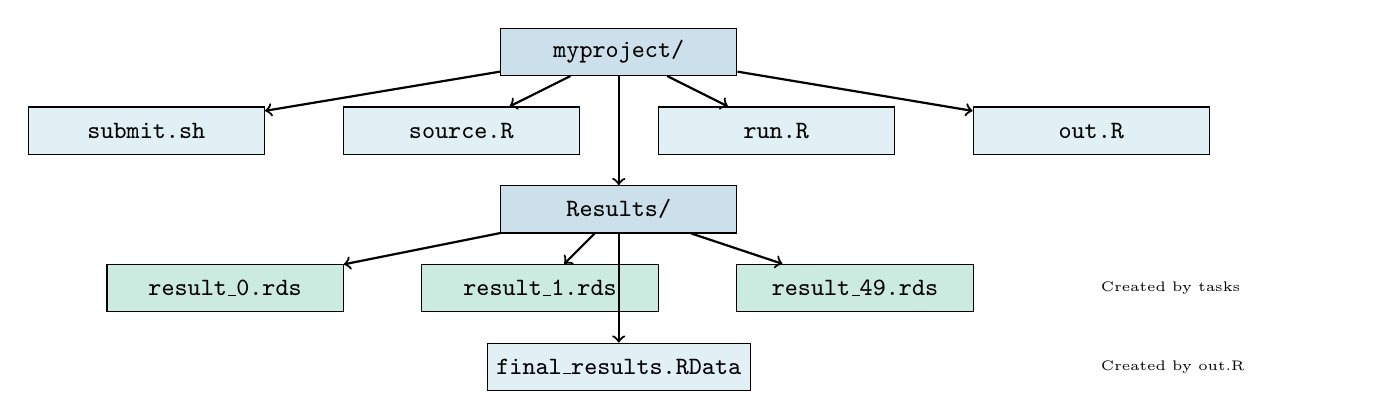
\begin{tikzpicture}[
    every node/.style={draw, rectangle, minimum width=3cm, minimum height=0.6cm, font=\small},
    folder/.style={fill=ceciblue!20},
    file/.style={fill=cecilight!20},
    result/.style={fill=accentgreen!20}
]
\node[folder] (proj) at (0,0) {\texttt{myproject/}};
\node[file] (submit) at (-6,-1) {\texttt{submit.sh}};
\node[file] (source) at (-2,-1) {\texttt{source.R}};
\node[file] (run) at (2,-1) {\texttt{run.R}};
\node[file] (out) at (6,-1) {\texttt{out.R}};

\node[folder] (results) at (0,-2) {\texttt{Results/}};
\node[result] (r0) at (-5,-3) {\texttt{result\_0.rds}};
\node[result] (r1) at (-1,-3) {\texttt{result\_1.rds}};
\node[result] (r49) at (3,-3) {\texttt{result\_49.rds}};

\node[file] (final) at (0,-4) {\texttt{final\_results.RData}};

\draw[->, thick] (proj) -- (submit);
\draw[->, thick] (proj) -- (source);
\draw[->, thick] (proj) -- (run);
\draw[->, thick] (proj) -- (out);
\draw[->, thick] (proj) -- (results);
\draw[->, thick] (results) -- (r0);
\draw[->, thick] (results) -- (r1);
\draw[->, thick] (results) -- (r49);
\draw[->, thick] (results) -- (final);

%\node[right, draw=none, text width=3cm, font=\tiny] at (6,-1) {Your 4 core files};
\node[right, draw=none, text width=3cm, font=\tiny] at (6,-3) {Created by tasks};
\node[right, draw=none, text width=3cm, font=\tiny] at (6,-4) {Created by out.R};
\end{tikzpicture}
\end{center}

\vspace{0.5em}
\begin{alertblock}{Before Submitting}
Create the Results folder: \texttt{mkdir Results}
\end{alertblock}
\end{frame}


\end{document}